%%% PREAMBLE - Do not touch %%%%%%%%%%%%%%%%%%%%%%%%%%%%%%%%%%%%%%%%%%%%%%%%%%%%%%
\documentclass[10pt,twocolumn,letterpaper]{article}
\usepackage[utf8]{inputenc}
\usepackage[portuges,brazil,english]{babel}
\usepackage{bm}
\usepackage{model}
\usepackage{times}
\usepackage{epsfig}
\usepackage{graphicx}
\usepackage{amsmath}
\usepackage{amssymb}
\usepackage{color}
\usepackage[pagebackref=true,breaklinks=true,letterpaper=true,colorlinks,bookmarks=false]{hyperref}
\input{pics/abaco}

\cvprfinalcopy % *** Uncomment this line for the final submission
\def\httilde{\mbox{\tt\raisebox{-.5ex}{\symbol{126}}}}
\ifcvprfinal\pagestyle{empty}\fi


%%% Report beginning %%%%%%%%%%%%%%%%%%%%%%%%%%%%%%%%%%%%%%%%%%%%%%%%%%%%%%%%%%%%%%
\begin{document}

%%% Title and authors %%%%%%%%%%%%%%%%%%%%%%%%%%%%%%%%%%%%%%%%%%%%%%%%%%%%%%%%%%%%
\title {Predicting the number of shares of a social network with linear regression }
\author{Gustavo Ciotto Pinton, RA117136\thanks{Is with the Institute of Computing, University of Campinas (Unicamp). \textbf{Contact}: \tt\small{gustavociotto@gmail.com}}}

%%% Abstract %%%%%%%%%%%%%%%%%%%%%%%%%%%%%%%%%%%%%%%%%%%%%%%%%%%%%%%%%%%%%%%%%%%%%
\maketitle
\begin{abstract}
Baseando-se em dados reais da rede social Mashable \cite{database}, este relatório utiliza técnicas de regressão linear para predizer o número de compartilhamentos que uma eventual publicação teria a partir dos seus atributos. São exploradas técnicas de regularização e seleção de variáveis, e discutidas as escolhas de alguns parâmetros, tal como a taxa de aprendizado e a complexidade dos modelos propostos. A regressão linear foi obtida por dois métodos diferentes, sendo eles gradient descent e mínimos quadrados, cujos resultados são comparados posteriormente.
\end{abstract}

%%% Introduction %%%%%%%%%%%%%%%%%%%%%%%%%%%%%%%%%%%%%%%%%%%%%%%%%%%%%%%%%%%%%%%%%
\section{Introdução}
\label{intro}

A regressão linear consiste em uma técnica simples cujo objetivo é relacionar um conjunto de dados de entrada com os de saída através do uso de uma equação linear \(Y = \theta_0 + \theta_1X_1 + \theta_2X_2 + \ldots + \theta_NX_N\), em que \(Y\), \(X_i\) e \(\theta_i\) representam, respectivamente, a saída gerada pelo modelo a partir de um conjunto de atributos e os coeficientes da equação. A equação anterior é utilizada apenas para uma amostra singular, porém, como visto em aula, o principal aspecto que garante a qualidade de resultados obtidos por métodos de aprendizado de máquina é o grande volume de dados. Tendo isso em vista, um conjunto de \(M\) amostras de entrada descritas por \(N\) atributos é representado pela matriz \(\bm{x}_{N+1\times M}\). Da mesma maneira, os coeficientes da equação são representados pelo vetor \(\bm{\theta}\) de \(N+1\) elementos e a saída, pelo vetor \(\bm{y}\) de \(M\) valores, de forma a obter a equação vetorial \ref{lr}, logo abaixo.

\begin{equation}
\label {lr}
\bm{y} = \bm{\theta}^T\bm{x}
\end{equation}

A determinação das componentes de \(\bm{\theta}\) é realizada a partir da minimização da função de custo \(J(\bm{\theta}, \bm{x})\), descrita pela equação \ref{cost}, em que \(\bm{x}_ i\) corresponde à i-ésima amostra e \(t_ i\) ao \textit{target} que deseja-se atingir.

\begin{equation}
\label {cost}
J(\bm{\theta}, \bm{x}) = \frac{1}{2M} \displaystyle\sum_{i=1}^{M} \left(\bm{\theta}^T\bm{x}^{(i)} - \bm{t}^{(i)}\right)^2
\end{equation}

Os dados utilizados para a minimização \(\bm{x}\) e \(\bm{t}^{(i)}\) pertencem a um conjunto chamado \textbf{conjunto de treinamento}, enquanto que a validação dos parâmetros obtidos ocorre em um conjunto que recebe este mesmo nome. Um regra geral é separar 80\% dos dados disponíveis para treinamento e o restante, 20\%, para testes e validação.

A função de custo \(J(\bm{\theta}, \bm{x})\) possui a importante propriedade de ser \textbf{convexa} \cite{Bishop:2006:PRM:1162264}. Isso garante que ela não possui mínimos locais, exceto pelo global. Deste modo, dois métodos de minimização podem ser utilizados. O primeiro, chamado de \textbf{equação normal}, permite obter o \(\bm{\theta}\) ótimo a partir de uma única expressão, representada em \ref{normal}. Observa-se rapidamente que o ponto negativo desta abordagem é o cálculo da matriz inversa, cuja complexidade assimptótica de computação é \(\Theta(n^3)\), conforme visto em aula. Para a matrix \(\bm{x}^T\bm{x}\) de dimensão \(N+1 \times N+1\), portanto, o número de atributos \(N\) pode representar um impedimento para o uso desta técnica.

\begin{equation}
\label {normal}
\bm{\theta} = \left(\bm{x}^T\bm{x}\right)^{-1} \bm{x}^T \bm{t}
\end{equation}

O segundo método, chamado de \textbf{gradient descent}, é iterativo e não requer o cálculo de nenhuma matriz inversa. Derivando-se parcialmente a equação \ref{cost} em relação a \(\bm{\theta}_j\), obtém-se o coeficiente linear e portanto a direção que devemos tomar para nos aproximar do mínimo global. Repetindo o raciocínio para todos os parâmetros \(\bm{\theta}_j\), obtém-se à operação \ref{gd} que deve ser aplicada a cada um deles a cada iteração. Ressalta-se que \(\bm{x}_1 = 1\) para todo \(i\).

\begin{equation}
\label {gd}
\bm{\theta}_j = \bm{\theta}_j - \frac{\alpha}{M} \displaystyle\sum_{i=1}^{M} \left(\bm{\theta}^T\bm{x}^{(i)} - \bm{t}^{(i)}\right)\bm{x}_j^{(i)}
\end{equation}

A equação \ref{gd} introduz o parâmetro \(\alpha\), chamado de \textit{learning rate}. Tal parâmetro controla a velocidade de convergência ao mínimo global, isto é, quanto maior o seu valor mais rapidamente ele é atingido. Por outro lado, valores muito grandes produzirão um efeito denominado \textit {overshooting}, isto é, a solução encontrada sempre ficará \textit{balançando} ao redor do mínimo sem nunca atingí-lo. Nas próximas seções, o autor explica a estratégia para a definição desta grandeza para o problema deste relatório.

Tendo visto toda teoria por trás da regressão linear, podemos aplicá-la a dados reais. Neste relatório, usamos dados reais \cite{database} da rede social \textit{Mashable}, que visam relacionar uma série de atributos de uma determinada publicação com o número de \textit{shares} que ela recebeu. Em outras palavras, busca-se encontrar uma relação linear entre o número de \textit{shares} recebidos com os atributos de uma publicação. No total, 31715 dados foram usados para treinamento dos modelos e 7929 para teste e validação.

%%% Add section %%%%%%%%%%%%%%%%%%%%%%%%%%%%%%%%%%%%%%%%%%%%%%%%%%%%%%%%%%%%%%%%%%
\section{Atividades}

As próximas subseções visam explicar as escolhas dos diversos parâmetros adotados pelo autor.

\subsection{Ajuste do learning rate}

Conforme mencionado na seção \ref{intro}, o parâmetro \textit{learning rate} controla a velocidade de convergência ao mínimo global da função de custo. Tendo em vista as questões levantadas nesta mesma seção, adota-se um valor \(\alpha\) inicial igual a 0.5, modificando-o em apenas duas situações:

\begin{itemize}
	\item Quando o erro da iteração \(k\) é superior aquele da iteração \(k -1\). Neste caso, conclui-se que a solução encontrada foi pior e, portanto, devemos diminuir a velocidade de convergência.
	\item A variação do erro entre as iterações \(k\) e \(k -1\), isto é, \(\frac{R_{k - 1} - R_k}{R_k}\), foi inferior a uma porcentagem \(\Delta = 0.5\%\). Neste caso, deseja-se eliminar os efeitos de \textit{overshooting} e aproximar o melhor possível do mínimo global. Denota-se de \(R_k\), dado pela fórmula \ref {rms}, o \textit{root-mean-square error} obtido na iteração \(k\):
	\begin {equation}
	\label{rms}
	R_k = \sqrt{\frac {\sum_{i=1}^{M} \left(\bm{\theta}^T\bm{x}^{(i)} - \bm{t}^{(i)}\right)^2}{M}}
	\end{equation}
\end{itemize}

Nestes dois casos, o valor de \(\alpha\) é diminuído pela metade.

\subsection {Ajuste das variáveis discretas}

A descrição dos atributos de cada uma das entradas revelou a presença de algumas variáveis discretas. Dois grupos foram identificados: um com variáveis do tipo \textit{a publicação ocorreu na segunda-feira?}, \textit{a publicação ocorreu na terça-feira?} e assim por diante, e outro com atributos semelhantes a \textit{o canal é de entretenimento?}. Duas abordagens foram simuladas para estes casos: a primeira foi simplesmente não realizar nenhuma transformação às variáveis e associar um \(\bm{\theta}_j\) a cada uma delas no modelo. A segunda, por sua vez, consistiu em transformar cada grupo em apenas um atributo a partir de potências de 2, isto é, ele será ascrescido de \(2^k\) se a k-ésima variável do grupo valer 1.

Os dois modelos foram testados, porém nenhum deles se destacou em termos dos erros de teste. Dessa forma, por apresentar um número menor de atributos, os resultados apresentados nas seções correspondem à \textbf{segunda abordagem apresentada}.

\subsection {Normalização dos dados de entrada e de saída}

A normalização dos dados antes do treinamento previne que os valores \(\bm{\theta}_j\) sejam extremamente pequenos ou grandes de forma a
causar instabilidades ou interferir na velocidade de convergência do modelo. Dentre as muitas maneiras de normalização que podem ser aplicadas, escolhemos para esta atividade aquela da equação \ref{norm}. Neste caso, são calculados a média \(\mu_j\) e o desvio padrão \(\sigma_j\) de cada \textit{feature} \(\bm {x'}_j\) sobre todas as amostras de treinamento e depois é aplicada a expressão \ref{norm}.

\begin {equation}
\label {norm}
\bm {x'}_j = \frac {\bm{x}_j - \mu_j}{\sigma_j}
\end{equation}

Vale lembrar que os valores \(\mu_j\) e \(\sigma_j\) devem ser amarzenados para serem utilizados posteriormente no conjunto de teste e em qualquer outra entrada a ser aplicada no modelo.

\subsection{Regularização}

A regularização é uma técnica que permite limitar os efeitos negativos de \textit{overfitting} sem a eliminação de nenhum atributo do modelo a partir da penalização dos parâmetros \(\bm{\theta}_j\). Neste caso, a equação \ref{cost} torna-se:

\begin{equation}
\label {cost-reg}
J(\bm{\theta}, \bm{x}) = \frac{1}{2M} \left[\displaystyle\sum_{i=1}^{M} \left(\bm{\theta}^T\bm{x}^{(i)} - \bm{t}^{(i)}\right)^2 + \lambda \displaystyle\sum_{j=2}^{N + 1} \bm{\theta}_j^2 \right]
\end{equation}

Observa-se que se \(\lambda\) é muito grande, então o processo de minimização produzirá \(\bm{\theta}_j\) pequenos, resultando em um modelo \textit{biased}. Em oposição, \(\lambda\) pequenos não conseguiriam combater os efeitos de \textit{overfitting} e a variação criada pelos dados de testes seria grande. Como mostrado na próxima seção, como não verificamos \textit{overfitting} durante os testes, atribui-se um valor pequeno a \(\lambda\), isto é, 0.8.

A equação \ref{norm}, por sua vez, transforma-se na expressão \ref{normal-reg}, sendo \(\bm{I}_{N \times N}\) a matriz identidade:

\begin{equation}
\label {normal-reg}
\bm{\theta} = \left(\bm{x}^T\bm{x} + \lambda
\begin{bmatrix}
    0       & 0 \\
    0       & \bm{I}_{N \times N} \\
\end{bmatrix}
\right)^{-1} \bm{x}^T \bm{t}
\end{equation}

Destaca-se que \(\bm{\theta}_1\) não é penalizado.

%%% Add section %%%%%%%%%%%%%%%%%%%%%%%%%%%%%%%%%%%%%%%%%%%%%%%%%%%%%%%%%%%%%%%%%%
\section{Soluções propostas}

Essa seção é dedicada à discussão das soluções propostas. Foram realizados testes com modelos simples, regularizados e contendo variáveis de segunda e terceira ordens.

\subsection {Modelo linear simples}

Neste modelo, utiliza-se o método de regressão linear sem regularização e sem quaisquer termos de segunda ou terceira ordens. Para a técnica de \textit{gradient descent}, itera-se a fórmula \ref{gd} 100 vezes no total. A figura \ref{fig:lr-gd} representa os erros quadrados médios conforme equação \ref{rms} obtidos no treinamento e no teste a cada iteração. Observa-se que ambos os erros se estabilizam em torno de, respectivamente, 10750 e 14600, e que não há a presença dos efeitos negativos de \textit {overfitting}.

\begin{figure}
    \centering
    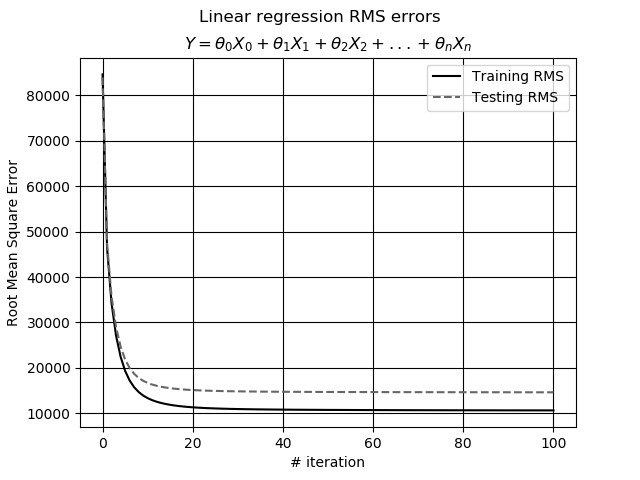
\includegraphics[width=0.9\columnwidth]{img/lr-gd.png}
    \caption{RMS obtidos no treinamento e teste a cada iteração.}
    \label{fig:lr-gd}
\end{figure}

A figura \ref{fig:lr-norm}, por sua vez, representa os resultados encontrados a partir do uso da expressão \ref{norm}. Dois gráficos são mostrados: no primeiro, compara-se os erros obtidos no treinamento e teste para diversos tamanhos de conjuntos de entrada indo de 10000 até 31715, enquanto que no segundo, compara-se os vetores \(\bm{\theta}\) obtidos pelos dois métodos descritos nessa seção. Conforme esperado, o RMS encontrado para o método normal, em torno de 10590, foi inferior aquele encontrado por \textit{gradient descent}. Observa-se também que as diferenças entre os vetores \(\bm{\theta}\) tendem a aumentar com o tamanho do conjunto de entrada.

\subsection{Modelo linear simples regularizado}

\subsection{Modelo linear de segunda ordem}

\subsection{Modelo linear de terceira ordem}

\begin{figure}
    \centering
    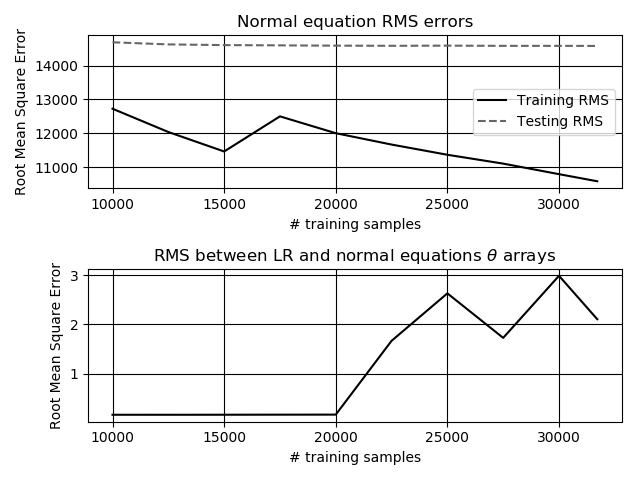
\includegraphics[width=0.9\columnwidth]{img/lr-norm.png}
    \caption{RMS obtidos no treinamento e teste para diversos números de amostras.}
    \label{fig:lr-norm}
\end{figure}

%%% Add section %%%%%%%%%%%%%%%%%%%%%%%%%%%%%%%%%%%%%%%%%%%%%%%%%%%%%%%%%%%%%%%%%%
\section{Experiments and Discussion}

%%% Add section %%%%%%%%%%%%%%%%%%%%%%%%%%%%%%%%%%%%%%%%%%%%%%%%%%%%%%%%%%%%%%%%%%
\section{Conclusions and Future Work}

%%% References %%%%%%%%%%%%%%%%%%%%%%%%%%%%%%%%%%%%%%%%%%%%%%%%%%%%%%%%%%%%%%%%%%%
{\small
\bibliographystyle{unsrt}
\bibliography{refs}
}

\end{document}
